\documentclass[11pt,a4paper]{report}

\usepackage{amssymb,amsmath,epsfig,float,subfig,hyperref,multicol}
\usepackage{pgfplots}
\usepgfplotslibrary{fillbetween}
\usepackage{xcolor}

\definecolor{SCSUred}{HTML}{CD1041}

\hypersetup{colorlinks=true,linkcolor=SCSUred,urlcolor=SCSUred}

\usepackage{enumerate}
\usepackage{tikz}
\usetikzlibrary{arrows}
\usetikzlibrary{patterns}
\usetikzlibrary{decorations}
%%\usetikzlibrary{intersections}
\usetikzlibrary{matrix}
\usetikzlibrary{snakes}
\usetikzlibrary{calc}
\usetikzlibrary{backgrounds}

\definecolor{linecolor}{HTML}{0074C8}
\definecolor{linecolor2}{HTML}{C80200}

\newcommand{\imagebullet}[1]{\includegraphics[width=0.5cm]{#1}}

\pagestyle{empty}
\setlength{\textwidth}{7in}
\setlength{\textheight}{10in}
\setlength{\oddsidemargin}{-25pt}
\setlength{\evensidemargin}{-25pt}
\setlength{\topmargin}{-50pt}

\usepackage[english]{babel}
\usepackage[utf8]{inputenc}
\usepackage{fancyhdr}
 
%%\pagestyle{fancy}
\renewcommand{\headrulewidth}{0pt}
%%\fancyhf{}
%%\rhead{Share\LaTeX}
%%\lhead{Guides and tutorials}
%%\cfoot{OVER}

\newcommand{\DueA}{Monday, November 18}
\newcommand{\DueB}{Tuesday, November 19}
\newcommand{\DueC}{Tuesday, November 26}

\begin{document}

\begin{figure}[ht]
\begin{flushright}
	\includegraphics[width=2.0in]{U_PriHorz_WhtLtBG.jpg}
	\end{flushright}
\end{figure}

\vspace{-12mm}

\begin{flushleft}
\Large\bf \href{https://activecalculus.org/single/sec-4-4-FTC.html}{4.4 - The Fundamental Theorem of Calculus}\rm
%%Daily Preparation - \DueA \rm
\end{flushleft}


\vspace{8pt}

\noindent {\Large\bf{Overview}} \\
In this section we see how antiderivatives allow us to compute a definite integral using the The Fundamental Theorem of Calculus. In this result, we see formally how the net-signed area under a curve is connected to the antiderivative of the function that generates the curve. This result extends our earlier work where we saw that slopes on the graph of $f$ generate heights on the graph of $f'$; now we can also see that net-signed areas between $f'$ and the $x$-axis are connected to differences in heights on $f$.


\vspace{16pt}

%%\pagebreak

\noindent {\Large\bf{To prepare for class}} \\
Complete all actions listed below.  Respond to the questions highlighted with {\color{SCSUred}{\boxed{Submit}}}.  %% by the start of class on {\bf{\DueA}}.  A single .pdf should be uploaded to D2L Brightspace.
\begin{itemize} \itemsep -2pt % Reduce space between items

\item {\bf{Read}} motivating questions and the introduction to \href{https://activecalculus.org/single/sec-4-4-FTC.html#LCP}{section 4.4} (up until Preview Activity 4.4.1).

\item {\bf{Do}} \href{https://activecalculus.org/single/sec-4-4-FTC.html#ZAQ}{Preview Activity 4.4.1}. 
\begin{itemize}\itemsep -2pt % Reduce space between items
\item (Optional) {\bf{Watch}} \href{https://www.youtube.com/watch?v=wIEk58A_6TU&t=422s}{video solution of Preview Activity 4.4.1 (8:24)}.
\item (Optional) Solutions to the Preview Activity 4.4.1 appear at the end of this document.  
\end{itemize}

\item {\bf{Watch}} video \href{https://www.youtube.com/watch?v=bwjUioJyWe8&feature=emb_title}{Quick Review - The Fundamental Theorem of Calculus (3:14)}.  

\item {\bf{Read}} \href{https://activecalculus.org/single/sec-4-4-FTC.html#rJY}{section 4.4.1} up to Activity 4.4.2. 

\item[\imagebullet{CopilotLogo.jpg}] Prompt {\bf{Copilot}} ``How is the fundamental theorem of calculus related to finding distance traveled by finding area under a velocity curve?"

\item[{\color{SCSUred} \boxed{Submit}}]  {\bf{Watch}} video \href{https://www.youtube.com/watch?v=1uxPq8Gtm18&feature=emb_title}{Fundamental Theorem of Calculus with Power Functions (7:32)}.   Note that the presenter does a terrible job in evaluation of $\displaystyle \int_{-1}^3 3x^2 - 2x + \pi \ dx$ by not using any = signs in the presentation.  Correct this by carefully writing the solution properly using appropriate notation (i.e. use equality signs as needed). 
 

\item {\bf{Do}} these problems.
\begin{enumerate}
\setcounter{enumi}{0}
\item Evaluate $\displaystyle \int_0^1 1-x^2 \ dx$.  Sketch a graph with the shaded region the answer represents.  Does your answer appear to be reasonable?

\item[\imagebullet{CopilotLogo.jpg}] Prompt {\bf{Copilot}} ``Evaluate \$\textbackslash int\_0$\wedge$1 1-x$\wedge$2 dx\$.   Then, produce and execute python code that will sketch a graph with the shaded region the answer represents."

\item 
\begin{enumerate}
\item Use geometry to evaluate $\displaystyle \int_{-1}^4 1-\frac{1}{2}x \ dx$.
\item Use the Fundamental Theorem of Calculus to evaluate this definite integral.  Note that you should get the same numerical value!
\end{enumerate}
\item Evaluate $\displaystyle \int_0^{\pi/2} \cos x \ dx$.  Sketch a graph with the shaded region the answer represents.  Does your answer appear to be reasonable?  {\it{Hint: What function has derivative of $\cos x$?  }}

\end{enumerate}


\item[{\color{SCSUred} \boxed{Submit}}] {\bf{Explore}} the applet \href{https://www.desmos.com/calculator/9nc0zu02l4}{1st Fundamental Theorem} built in Desmos.  The applet shows that the area under a curve defined by $f(x)$ (shaded blue) is equal to the difference in heights $F(b)-F(a)$ of an antiderivative $F(x)$ at the endpoints $a$ and $b$.  Then, draw your own well-labeled figure illustrating this idea for $\displaystyle \int_{-1}^2 3x^2 \ dx = 8-(-1)=9$.  Be sure that your figure (a) clearly shades the area being computed, (b) contains graphs of both $f(x)$ and antiderivative $F(x)$, and (c) shows the difference in heights $F(b)-F(a)$.  



\item {\bf{Read}} \href{https://activecalculus.org/single/sec-4-4-FTC.html#XRh}{section 4.4.2}.  

\item {\bf{Watch}} video \href{https://www.youtube.com/watch?v=SafcRvQKe4g&feature=emb_title}{Fundamental Theorem of Calculus with Exponential Functions (7:56)}. 

\item {\bf{Do}} these problems.
\begin{enumerate}
\setcounter{enumi}{3}
\item 
\begin{enumerate}
\item Use the Fundamental Theorem of Calculus to evaluate $\displaystyle \int_2^4 e^x \ dx$.  
\item  Calculate $\displaystyle \int_0^1 2xe^{x^2} \ dx$ two ways: (i) numerically using {\it{GeoGebra}} and (ii) exactly using the fundamental theorem of calculus.  How do these values compare?  
\item Give examples of two different functions $f(x)$ and limits of integration $a$ and $b$ such that $\displaystyle \int_a^b f(x) \ dx = e^4 - e^2$. 
\end{enumerate}
\item Find two antiderivatives of $g(x) = \sec x \tan x$. 



\end{enumerate}
 

\item[{\color{SCSUred} \boxed{Submit}}] {\bf{Explore}} the applet \href{https://www.geogebra.org/m/WjhEpeNd}{Practice Applying the Fundamental Theorem of Calculus} by trying a few of these by hand and checking that you get the same result.  Take a screen capture of one problem it presents and submit with it your written work showing that you get the same result.  


\end{itemize}













\vspace{16pt}

\noindent {\Large\bf{After class}}\\
Solidifying the concepts discussed in class through practice is necessary to build your skills. 

%%\noindent {\large\bf{After \DueA}}
\begin{itemize}\itemsep -2pt % Reduce space between items
\item {\bf{Do}} \href{https://activecalculus.org/single/sec-4-4-FTC.html#HHd}{exercises 1-6 in section 4.4}.

%%\item {\bf{Do}} \href{https://activecalculus.org/single/sec-4-4-FTC.html#ovP}{Activity 4.4.3}. 

\item {\bf{Read}} \href{https://activecalculus.org/single/sec-4-4-FTC.html#DYq}{section 4.4.3}.

\item {\bf{Watch}} video \href{https://www.youtube.com/watch?v=Q8ZKTA4w9q0&list=PL9bIjQJDwfGuXQHuS5Jkmum_CFILoCZX-&index=91}{Applications of the Total Change Theorem (6:40)}.   



 
\item {\bf{Do}} \href{https://activecalculus.org/single/sec-4-4-FTC.html#VRM}{exercises 7-8 in section 4.4}.

%%\end{itemize}

%%\noindent {\large\bf{After \DueB}}
%%\begin{itemize}\itemsep -2pt % Reduce space between items

\item {\bf{Read}} \href{https://activecalculus.org/single/sec-4-4-FTC.html#kfz}{section 4.4.4 - summary}.

%%\item {\bf{Do}} \href{https://activecalculus.org/single/sec-4-3-definite-integral.html#AMl}{WebWork exercises 3-6 in section 4.3}. 

\item {\bf{Do}} \href{https://activecalculus.org/single/sec-4-4-FTC.html#BYV}{exercises 8-10 in section 4.4}.

\item {\bf{Start working}} on the \href{https://www.myopenmath.com/index.php}{MOMwork} (MyOpenMath) assignment for this section.  %%This will be due on \DueC. 

\end{itemize}


%%\pagebreak

\vspace{16pt}

\noindent {\Huge\bf{Extra Prep}}

\vspace{16pt}

\noindent {\Large\bf{Basic learning objectives}}\\
These are the tasks you should be able to perform with reasonable
fluency when you arrive at our next class meeting. Important new
vocabulary words are indicated {\it{in italics}}.  Check each box when you feel confident you have a firm grasp on that objective.  

\begin{itemize} \itemsep -2pt % Reduce space between items
\renewcommand{\labelitemi}{\scriptsize$\square$}
\item Recognize that the change in position of an object gives the net-signed area bounded by a velocity curve on an interval $[a,b]$: $\int_a^b v(t) \ dt = s(b)-s(a)$.

\item Define an {\it{antiderivative}}.

\item State the Fundamental Theorem of Calculus: $\int_a^b f(x) \ dx=F(b)-F(a)$, where $F$ is any antiderivative of $f$.

\item Apply the Fundamental Theorem of Calculus to compute definite integrals. %%where the integrand is a sum or difference of terms with power or exponential functions.
\end{itemize}

\vspace{16pt}

\noindent {\Large\bf{Advanced learning objectives}}\\
In addition to mastering the basic objectives, here are the tasks you should be able to perform after class, with practice:
\begin{itemize} \itemsep -2pt % Reduce space between items
\renewcommand{\labelitemi}{\scriptsize$\square$}
\item Compute the family of antiderivatives of a function.
\item Explain why two antiderivatives of the same function only differ by a constant.
\item State the Total Change Theorem and explain it's relationship to the Fundamental Theorem of Calculus.
\item Apply the Total Change Theorem to solve applied problems.
\end{itemize}

\vspace{16pt}

\noindent {\Large\bf{Need More Help?}}

\begin{itemize}\itemsep -2pt % Reduce space between items

\item  {\bf{Watch}} video \href{https://www.youtube.com/watch?v=hIJHRr4YOg0&feature=youtu.be}{Antiderivatives Part I - Polynomials and the Power Rule (8:22)}. 

\item  {\bf{Watch}} video \href{https://www.youtube.com/watch?v=AeASWdqiDv0&feature=youtu.be}{First Fundamental Theorem of Calculus (8:00)}.  

\item  {\bf{Watch}} video \href{https://www.youtube.com/watch?v=WgKXMKf7opE&feature=youtu.be}{Antiderivatives Part II - 1/x, Exponentials, and Trig Functions (6:21)}.

\item  {\bf{Explore}} another good applet illustrating the \href{https://www.geogebra.org/m/r4A2xSSp#material/kwaegjvp}{Fundamental Theorem of Calculus Part 1}.  

\item {\bf{Do}} these problems.
\begin{enumerate}
\setcounter{enumi}{5}

\item Find a single antiderivative for each of the following functions.  In each case, you will want to reverse the chain rule.    
\begin{enumerate}
\item $\displaystyle f(x) = \cos (3x)$
\item $\displaystyle g(x) = 2\sin(x)\cos(x)$
\item $\displaystyle h(x) = \sin (2x)$
\end{enumerate} 

\item Suppose you know that a certain function $f$ is twice differentiable and that its
graph over $[-4,8]$ is given in the figure below.  As you see, the printer was sloppy and 
spilled a lot of ink on the graph.  Using the Fundamental Theorem of Calculus, decide whether each of the following definite
integrals is positive, negative, or zero.  Defend your answers.  
\begin{enumerate}
\item $\displaystyle{\int_{-2}^6f''(x)\  dx}$

\item $\displaystyle{\int_{-2}^6f'(x) \ dx}$
\end{enumerate}


\begin{figure}[H]
\centering
{
  \begin{tikzpicture}[thick,scale=0.75]
\draw[step=1cm,color=gray!50] (-5,-5) grid (9,5);
   \draw [black!80,line width=0.3pt,-latex] (0,0) -- (9,0) node [below] at (8.75,0) {$x$};
   \draw [black!80,line width=0.3pt,-latex] (0,0) -- (-5,0);
   \draw [black!80,line width=0.3pt,-latex] (0,0) -- (0,5) node [right] at (0,4.75) {$y$};
   \draw [black!80,line width=0.3pt,-latex] (0,0) -- (0,-5.0);
\draw[color=linecolor, line width=1pt,domain=-4:8,smooth]   plot (\x,{0.5*(2+(0.25*\x*\x-\x+2)*sin(2*180/3.14*\x))}) node [left] at (6.75,3.5) {$f(x)$};

\fill [black] (2,1) circle (1cm);
\fill [black] (0,1) circle (0.35cm);
\fill [black] (3,1.25) circle (0.5cm);
\fill [black] (1,-1.25) circle (0.65cm);
\fill [black] (-4,-1.75) circle (1cm);

\foreach \x/\xtext in {-4/-4, -2/-2, 2/2, 4/4, 6/6, 8/8}
    \draw[shift={(\x,0)}] (0pt,3pt) -- (0pt,-3pt) node[below] {$\xtext$};
\foreach \y/\ytext in {-4/-16, -3/-12, -2/-8, -1/-4, 1/4, 2/8, 3/12, 4/16}
    \draw[shift={(0,\y)}] (-2pt,0pt) -- (2pt,0pt) node[left] {$\ytext$};
\end{tikzpicture}}  
\end{figure}
\end{enumerate}

\item  {\bf{Do}} \href{https://activecalculus.org/single/sec-4-4-FTC.html#HTh}{Activity 4.4.4}.
\begin{itemize}
\item  {\bf{Watch}} video \href{https://www.youtube.com/watch?v=BK-OBadYgVs}{solution to (a) and (b) to Activity 4.4.4 (3:27)}.  
\item  {\bf{Watch}} video \href{https://www.youtube.com/watch?v=0J6lZPmYbaQ}{solution to (c) and (d) of Activity 4.4.4 (5:34)}. 
\end{itemize} 
\end{itemize}



\vspace{16pt}

\pagebreak

\noindent {\Large\bf{Selected Answers}}
\begin{enumerate}
\setcounter{enumi}{0}
\item[] \href{https://activecalculus.org/single/sec-4-4-FTC.html#ZAQ}{Preview Activity 4.4.1}
\begin{enumerate}[(a)]
\item $s(t) = -16t^2 + 16t+32$
\item Maximum height is at time $t=1/2$ second.  It lands at time $t=2$ seconds.
\item $s(\frac{1}{2})-s(0)=4$ feet; $s(2)-s(\frac{1}{2}) = -36$ feet; $s(2)-s(0)=-32$ feet. The first value represents the distance the balloon traveled upward from launch until it reached it's peak.  The second value represents the (signed) distance the balloon traveled from peak until hitting the ground (i.e. the displacement).  The third value represents the displacement of the balloon from launch until hitting the ground.  
\item 40 feet
\item The total net signed area is 4-36=-32.

\vspace{-15mm}
\begin{figure}[H]
\flushright
{
  \begin{tikzpicture}[thick,scale=1.0]
      \fill [linecolor!20] (0,0) -- (0.5,0) -- (0,1.6) -- (0,0);
    %%\draw[black] (0.5,0) -- (0.5,1.778) -- (2,1.778) -- (2,0) -- (0.5,0);
      \fill [red!20] (0.5,0) -- (2,0) -- (2,-4.8) -- (0.5,0);
    %%\draw[black] (2,0) -- (2,1.067) -- (3.5,1.067) -- (3.5,0) -- (2,0);
      %%\fill [linecolor!20] (3.5,0) -- (3.5,0.762) -- (5,0.762) -- (5,0) -- (3.5,0);
    %%\draw[black] (3.5,0) -- (3.5,0.762) -- (5,0.762) -- (5,0) -- (3.5,0);
%%\draw[step=1cm,color=gray!50,dotted] (0,-3) grid (5,3);
   \draw [black!80,line width=0.3pt,-latex] (0,0) -- (2.5,0) node [below] at (2.25,0) {$t$};
   \draw [black!80,line width=0.3pt,-latex] (0,0) -- (-0.5,0);
   \draw [black!80,line width=0.3pt,-latex] (0,0) -- (0,2.5) node [right] at (0,2.25) {$v$};
   \draw [black!80,line width=0.3pt,-latex] (0,0) -- (0,-5.5);
\draw[color=linecolor, line width=1pt,domain=0:2]   plot (\x,{-3.2*\x+1.6}) node [above] at (2,-3) {$\displaystyle v(t)$};
%%node [right] at (3,3) {$y=1-x^2$};
\foreach \x/\xtext in { 1/1, 2/2}
    \draw[shift={(\x,0)}] (0pt,3pt) -- (0pt,-3pt) node[below] {$\xtext$};
\foreach \x/\xtext in {1,  2}
    \draw[shift={(\x,0)}] (0pt,1.5pt) -- (0pt,-1.5pt);
%% node[below] {$\xtext$};
\foreach \y/\ytext in {-5/-50,-4/-40, -3/-30,-2/-20, -1/-10, 1/10, 2/20}
    \draw[shift={(0,\y)}] (-2pt,0pt) -- (2pt,0pt) node[left] {$\ytext$};
\end{tikzpicture}}  
\end{figure}

\end{enumerate}

\vspace{-50mm}
\item 2/3 is a reasonable answer for the area of the shaded region.  

\begin{figure}[H]
\flushleft
{
  \begin{tikzpicture}[thick,scale=1.25]
  \fill[color=linecolor!20, line width=1pt,domain=0:1]   plot (\x,{1-\x*\x}) -- (1,0) -- (0,0);
      %%\fill [linecolor!20] (0,0) -- (0.5,0) -- (0,1.6) -- (0,0);
    %%\draw[black] (0.5,0) -- (0.5,1.778) -- (2,1.778) -- (2,0) -- (0.5,0);
      %%\fill [red!20] (0.5,0) -- (2,0) -- (2,-4.8) -- (0.5,0);
    %%\draw[black] (2,0) -- (2,1.067) -- (3.5,1.067) -- (3.5,0) -- (2,0);
      %%\fill [linecolor!20] (3.5,0) -- (3.5,0.762) -- (5,0.762) -- (5,0) -- (3.5,0);
    %%\draw[black] (3.5,0) -- (3.5,0.762) -- (5,0.762) -- (5,0) -- (3.5,0);
%%\draw[step=1cm,color=gray!50,dotted] (0,-3) grid (5,3);
   \draw [black!80,line width=0.3pt,-latex] (0,0) -- (2,0) node [below] at (1.75,0) {$x$};
   \draw [black!80,line width=0.3pt,-latex] (0,0) -- (-1.5,0);
   \draw [black!80,line width=0.3pt,-latex] (0,0) -- (0,1.5) node [right] at (0,1.25) {$y$};
   \draw [black!80,line width=0.3pt,-latex] (0,0) -- (0,-1.5);
\draw[color=linecolor, line width=1pt,domain=-1:1.5]   plot (\x,{1-\x*\x}) node [right] at (0.5,1) {$\displaystyle f(x)=1-x^2$};
%%node [right] at (3,3) {$y=1-x^2$};
\foreach \x/\xtext in { 1/1, 2/2}
    \draw[shift={(\x,0)}] (0pt,3pt) -- (0pt,-3pt) node[below] {$\xtext$};
\foreach \x/\xtext in {1,  2}
    \draw[shift={(\x,0)}] (0pt,1.5pt) -- (0pt,-1.5pt);
%% node[below] {$\xtext$};
\foreach \y/\ytext in {-1/-1, 1/1}
    \draw[shift={(0,\y)}] (-2pt,0pt) -- (2pt,0pt) node[left] {$\ytext$};
\end{tikzpicture}}  
\end{figure}

\item  
\begin{enumerate}
\item 9/4-1=5/4; this is the signed area shown.
\vspace{-10mm}
\begin{figure}[H]
\flushright
{
  \begin{tikzpicture}[thick,scale=1] 
%%\draw[step=1cm,color=gray!50,dotted] (0,-3) grid (5,3);
  \fill[color=linecolor!20, line width=1pt,domain=-1:2]   plot (\x,{1-0.5*\x}) -- (2,0) -- (-1,0);
    \fill[color=red!20, line width=1pt,domain=2:4]   plot (\x,{1-0.5*\x}) -- (4,0) -- (2,0);
   \draw [black!80,line width=0.3pt,-latex] (0,0) -- (5,0) node [below] at (4.75,0) {$x$};
   \draw [black!80,line width=0.3pt,-latex] (0,0) -- (-1.5,0);
   \draw [black!80,line width=0.3pt,-latex] (0,0) -- (0,3) node [right] at (0,2.75) {$y$};
   \draw [black!80,line width=0.3pt,-latex] (0,0) -- (0,-1.5);
\draw[color=linecolor, line width=1pt,domain=-1:4]   plot (\x,{1-0.5*\x}) node [right] at (1,1) {$y=1-\frac{1}{2}x$};

\foreach \x/\xtext in { -1/-1, 1/1, 2/2, 3/3, 4/4}
    \draw[shift={(\x,0)}] (0pt,3pt) -- (0pt,-3pt) node[below] {$\xtext$};
\foreach \y/\ytext in {-1/-1, 1/1, 2/2}
    \draw[shift={(0,\y)}] (-2pt,0pt) -- (2pt,0pt) node[left] {$\ytext$};
\end{tikzpicture}}  
\end{figure} 

\item $\displaystyle \int_{-1}^4 1-\frac{1}{2}x \ dx = F(4)-F(1) = 5/4$ where $F(x) = x - \frac{1}{4}x^2$, for example.  
\end{enumerate}

\item $\sin(\frac{\pi}{2}) - \sin(0)=1$ is a reasonable answer for the area of the shaded region.  

\begin{figure}[H]
\flushleft
{
  \begin{tikzpicture}[thick,scale=1.25]
  \fill[color=linecolor!20, line width=1pt,domain=0:1.57]   plot (\x,{cos(\x*180/3.14)}) -- (1.57,0) -- (0,0);
      %%\fill [linecolor!20] (0,0) -- (0.5,0) -- (0,1.6) -- (0,0);
    %%\draw[black] (0.5,0) -- (0.5,1.778) -- (2,1.778) -- (2,0) -- (0.5,0);
      %%\fill [red!20] (0.5,0) -- (2,0) -- (2,-4.8) -- (0.5,0);
    %%\draw[black] (2,0) -- (2,1.067) -- (3.5,1.067) -- (3.5,0) -- (2,0);
      %%\fill [linecolor!20] (3.5,0) -- (3.5,0.762) -- (5,0.762) -- (5,0) -- (3.5,0);
    %%\draw[black] (3.5,0) -- (3.5,0.762) -- (5,0.762) -- (5,0) -- (3.5,0);
%%\draw[step=1cm,color=gray!50,dotted] (0,-3) grid (5,3);
   \draw [black!80,line width=0.3pt,-latex] (0,0) -- (3.5,0) node [below] at (3.25,0) {$x$};
   \draw [black!80,line width=0.3pt,-latex] (0,0) -- (-1.5,0);
   \draw [black!80,line width=0.3pt,-latex] (0,0) -- (0,1.5) node [right] at (0,1.25) {$y$};
   \draw [black!80,line width=0.3pt,-latex] (0,0) -- (0,-0.5);
\draw[color=linecolor, line width=1pt,domain=-1:3.25]   plot (\x,{cos(\x*180/3.14)}) node [right] at (0.5,1) {$\displaystyle f(x)=\cos x$};
%%node [right] at (3,3) {$y=1-x^2$};
\foreach \x/\xtext in { 1/1, 2/2}
    \draw[shift={(\x,0)}] (0pt,3pt) -- (0pt,-3pt) node[below] {$\xtext$};
\foreach \x/\xtext in {1,  2, 3}
    \draw[shift={(\x,0)}] (0pt,1.5pt) -- (0pt,-1.5pt);
%% node[below] {$\xtext$};
\foreach \y/\ytext in { 1/1}
    \draw[shift={(0,\y)}] (-2pt,0pt) -- (2pt,0pt) node[left] {$\ytext$};
\end{tikzpicture}}  
\end{figure}

\item  
\begin{enumerate}[(a)]
\item $\displaystyle \int_2^4 e^x \ dx = e^4 - e^2$
\item $\displaystyle \int_{0}^1 2xe^{x^2} \ dx = F(1)-F(0) = e^1-1$ where $F(x) = e^{x^2}$ is one antiderivative of $f(x) = 2xe^{x^2}$.  {\it{GeoGebra}} should estimate this to be 1.71.  
\item If $f(x) = e^x$, then $\displaystyle \int_2^4 e^x \ dx = e^4 - e^2$  If $g(x) = 2xe^{x^2}$, then $\displaystyle \int_{\sqrt{2}}^2 2xe^{x^2} \ dx = e^4 - e^2$ since $G(x) = e^{x^2}$ is one antiderivative of $g(x)$.  
\end{enumerate}

\item $G_1(x) = \sec x$ and $G_2(x)=\sec x + 7$ work.  

\item 
\begin{enumerate}[(a)]
\item $\displaystyle F(x) = \frac{1}{3} \sin(3x)$
\item $\displaystyle G(x) = (\sin x)^2$
\item $\displaystyle H(x) = -\frac{1}{2}\cos(2x)$
\end{enumerate}



\item 
\begin{enumerate}[(a)]
\item positive
\item negative
\end{enumerate}

\end{enumerate}

\end{document}















